%  Add 'draft' option to mark overfull boxes with black boxes
%  Add 'showkeys' option to make keywords appear
\documentclass[
aps,
reprint,
amsmath, amssymb,
%preprint,
superscriptaddress,
%groupedaddress
]{revtex4-2}
\usepackage[spanish]{babel}
\usepackage{float}
\usepackage{graphicx}
\usepackage{dcolumn}
\usepackage{bm}
\usepackage{physics}
\renewcommand{\andname}{y}
\renewcommand{\spanishtablename}{Tabla}
\begin{document}
\preprint{Universidad de Córdoba}
% Use the \preprint command to place your local institutional report number in the upper righthand corner of the title page in preprint mode.
%\preprint{}

%Title of paper
\title{Determinación Experimental de las leyes \\de la Reflexión y Refracción de luz}

\author{Luis Miguel Patiño Buendía}
\author{Jesús Manuel Gallego Mercado}

\affiliation{Universidad de Córdoba.\\ Montería-Córdoba, Colombia}

%\email[]{Your e-mail address}
%\homepage[]{Your web page}
%\thanks{}


\date{\today}

\begin{abstract}
En este informe de laboratorio se abordó experimentalmente el comportamiento de un rayo de luz que se propaga por el aire y se hace incidir sobre un segundo medio material como: un lente y un espejo, cada uno con características específicas. Esto con el objetivo de determinar algunas de las leyes de la óptica geométrica para el fenómeno de la reflexion y la refracción de la luz (vista en éste contexto como un rayo o haz rectilíneo) al interactuar con distintos medios de propagación. Para esto, se realizó un montaje que consistió en hacer incidir desde un foco luminoso, un rayo de luz ubicado a una distancia conocida. Primeramente; sobre un espejo plano ubicado sobre un disco de Hartl. Y luego, se realizó un segundo montaje similar, pero utilizando en este caso una sección de lente semicircular. En ambos experimentos se tomaron medidas angulares acerca de la dirección del haz de luz antes y después de incidir sobre la superficie que separa al segundo medio del primero. Se concluyó que cuando un haz de luz incide sobre una superficie que separa dos medios diferentes, el haz que se refleja y el haz incidente poseen la misma separación angular con respecto a un eje normal a la superficie y se obtuvo que la dirección de un haz que se propaga por un medio, al atravesar un segundo medio tendrá una dirección que depende de la razón entre los índices de refracción de los medios materiales y del ángulo del haz incidente.
\end{abstract}


%\keywords{}
\maketitle
% References should be done using the \cite, \ref, and \label commands
\section{Introducción}
El estudio sistemático de los fenómenos que experimenta la materia y su interacción diaria con el hombre, lo han llevado a la necesidad de entender de manera profunda y específica la manera en como estos funcionan, a fin de predecir el comportamiento del espacio en que habita. El propósito de esta práctica, radica en el estudio de la luz como Onda Electromagnética en el campo de la Óptica Geométrica. Más específicamente, estudiar las propiedades de \textit{Reflexión y Refracción} de un rayo de luz que incide con carcteristicas especificas y ''controladas'' a la hora de realizar el experimento.

\section{Reflexión y Refracción}
La reflexión y la refracción de la luz son dos fenómenos físicos que puede experimentar un rayo de luz. En la reflexión, el rayo de luz rebota sobre una superficie, mientras en la refracción el rayo de luz que pasa de un medio a otro cambia su ángulo de propagación.

\subsection{Reflexión de la Luz}

En la reflexión de la luz se puede distinguir el rayo original o rayo incidente y el rayo que se devuelve o rayo reflejado. En el punto donde el rayo incidente y el reflejado se encuentran, se traza una línea imaginaria perpendicular a la superficie que se conoce como normal.\\
\\
Entre el rayo incidente y la normal se forma el ángulo de incidencia, y entre la normal y el rayo reflejado se forma el ángulo de reflexión. Así, la dirección en que se refleja la luz depende de la forma de la superficie reflectante y de la dirección del rayo incidente \cite{optics}.\\
\\
\textbf{Leyes de la Reflexión de la Luz}

\begin{itemize}
    \item El rayo incidente, la normal a la superficie de incidencia y el rayo reflejado están en el mismo plano.
    
    \item  El ángulo de incidencia $\theta_{i} $ y el ángulo de reflexión $\theta_{r}$ son iguales, por lo que la luz será reflejada invirtiendo el sentido de la propagación.
\end{itemize}


\subsection{Refracción de la Luz}

La refracción de la luz se produce en la superficie de separación de los medios de diferente densidad;lo que afecta la velocidad de propagación de la luz. El desvío de la dirección de propagación será mayor a mayor diferencia de la velocidad de propagación en los dos medios.\\
\\
En la refracción de la luz se distingue el rayo incidente y el rayo refractado. Entre el rayo incidente y la línea normal se forma el ángulo de incidencia. Mientras que entre el rayo refractado y la normal se forma el ángulo de refracción \cite{optics}.\\


\textbf{Leyes de la Refracción de la Luz}

\begin{itemize}
    \item Los índices de refracción $n_1$ y $n_2$, el ángulo de incidencia $\theta_{i}$ y el ángulo del haz refractado o transmitido $\theta_{t}$ se relacionan por la siguiente expresión:
    
    \begin{equation}
        \label{eqn:ley_snell}
        n_{1} \sin{\theta_{i}} = n_{2} \sin{\theta_{t}} 
    \end{equation}
\end{itemize}

\section{Objetivos}
\begin{enumerate}
    \item Comprobar experimentalmente algunas de las leyes de la óptica geométrica.
    \begin{itemize}
        \item Observar la reflexión de la luz y comprobar la segunda ley de la reflexión.
        \item Observar el comportamiento de un rayo de luz que pasa de un medio homogéneo (aire) a otro distinto (como el vidrio) y con base en los resultados, establecer la ley de Snell.
    \end{itemize}
\end{enumerate}

\section{Experimento y Metodología}
\begin{table}
	\caption{\label{tab:materiales}Materiales e Instrumentos de medida.}
	\begin{ruledtabular}
		\begin{tabular}{lcc}
            \textrm{Materiales} & \textrm{Referencia} & \textrm{Cantidad}\\
			\colrule
            Banco Óptico                & --------- & 1\\
			Diafragma con una Ranura    & --------- & 1\\
            Disco de Hartl              & --------- & 1\\
            Foco Luminoso               & --------- & 1\\
            Lente de $f'=+50mm, 40\Phi$ & --------- & 1\\
            Sección de lente semicircular & --------- & 1\\
            $R=+25mm$      & &\\
            Soporte para foco y disco   & --------- & 2\\
            Soporte para diafragma      & --------- & 1\\
            Espejo                      & --------- & 1\\
            Transformador S. $12V-20W$  & --------- & 1\\
	\end{tabular}
	\end{ruledtabular}
\end{table}

El experimento se divividó en dos partes, cada una con un montaje similar pero con medios de propagación distintos:

\subsection{Reflexión de un haz de luz.}
Para esta sección se situó un foco luminoso sobre el banco óptico de modo que su filamento coincida con el cero de la escala del banco. Frente al foco, en la marca de $5 cm$ de la regla del banco, se colocó una lente de $f=50mm$. Seguidamente, se ubicó un diafragma con ranura frente a la lente, de modo que se obtuvieran rayos de luz paralelos. Delante del diafragma se colocó un disco de Hartl y sobre éste, un espejo plano que se alinea con el diámetro del disco $(90^{\circ}-90^{\circ})$.

Al conectar el foco luminoso, el disco de Hartl se acomodó de modo que se observara un rayo de luz nítido que coincida con el diámetro $(0^{\circ}-(180^{\circ})$, siendo el punto 0 el más próximo al foco de luz.

El montaje es tal y como se observa en la figura \ref{fig:img_0}. Se hicieron medidas del ángulo del haz incidente y del haz reflejado. La información se consignó en la sección \ref{sec:resultados}.

\begin{figure}
\centering
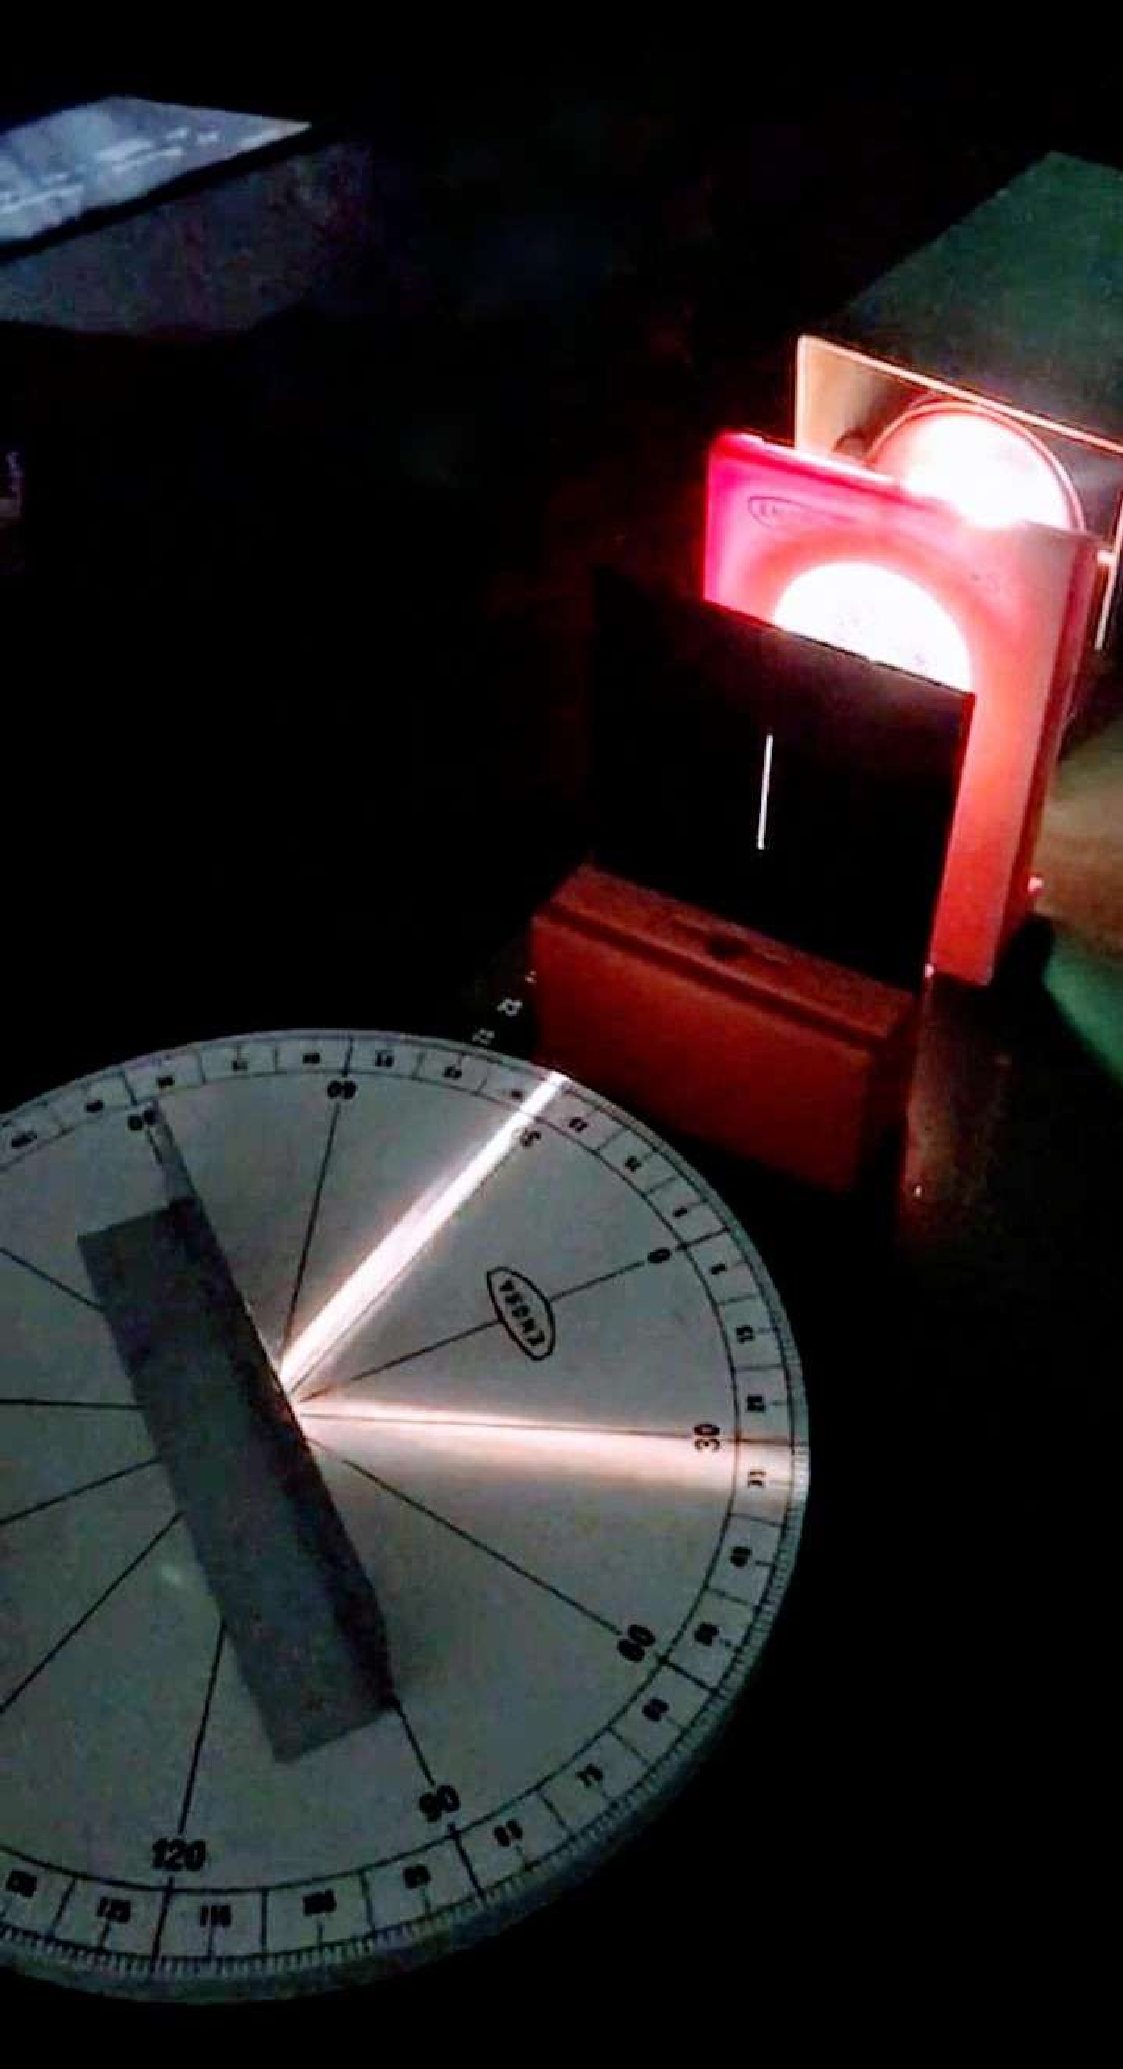
\includegraphics[width=0.5\columnwidth]{img/img0.pdf}
\caption{\label{fig:img_0} Montaje experimental: Reflexión de la luz.}
\end{figure}

\subsection{Refracción de un haz de luz}
En esta parte del experimento, se usó un montaje similar al anterior, excepto que en vez de colocar un espejo en el disco de Hartl, se ubicó una sección de lente semicircular con su cara plana mirando hacia el foco luminoso y coincidiendo con el diámetro $(90^{\circ}-(90^{\circ})$. El centro de la cara plana se hizo coincidir con el centro del disco. Seguidamente se giró cuidadosamente el disco sin mover la posición de la lente, provocando una separación angular entre el haz de luz y el eje normal a la cara plana del lente.
Se tomaron medidas del ángulo del haz incidente y el haz saliente (o refractado) con respecto a la normal.

\begin{figure}
\centering
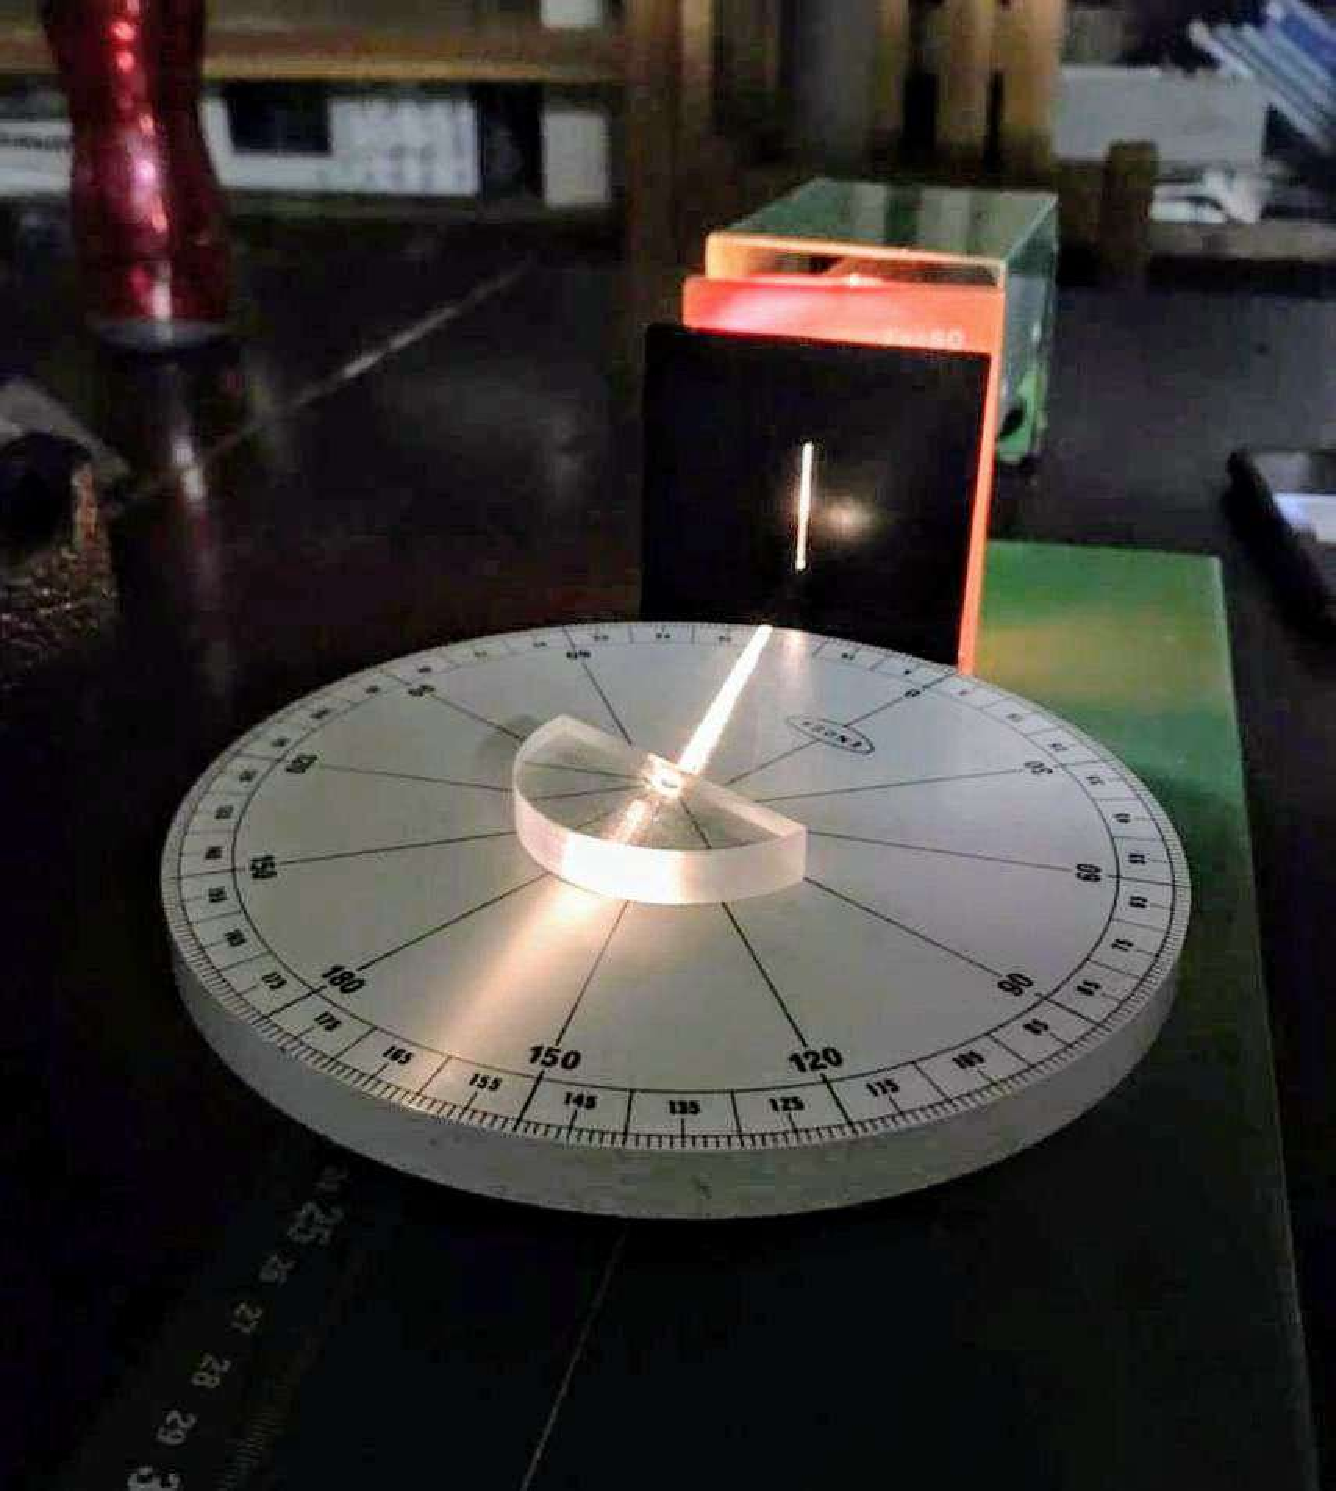
\includegraphics[width=0.5\columnwidth]{img/img1.pdf}
\caption{\label{fig:img_1} Montaje experimental: Refracción de la luz.}
\end{figure}

\section{\label{sec:resultados}Resultados}
\begin{table}[H]%[H] add [H] placement to break table across pages
    \caption{\label{tab:tabla1} Medidas angulares del experimento de la reflexión de la luz. Los ángulos se miden con respecto al eje normal a la superficie plana del espejo.}
     \begin{ruledtabular}
     \begin{tabular}{cc}
        Ángulo de Incidencia $(\theta_i)$ & Ángulo de Reflexión $(\theta_r)$ \\
        \hline
        30$^{\circ}$ & 28$^{\circ}$ \\
        45$^{\circ}$ & 42$^{\circ}$ \\
        60$^{\circ}$ & 57$^{\circ}$ \\
        75$^{\circ}$ & 71$^{\circ}$\\
        90$^{\circ}$ & 88$^{\circ}$
     \end{tabular}
     \end{ruledtabular}
\end{table}

\begin{table}[H]%[H] add [H] placement to break table across pages
    \caption{\label{tab:tabla2} Medidas angulares del experimento de refracción de la luz. Los ángulos se miden con respecto al eje normal a la superficie plana del material semicircular}
     \begin{ruledtabular}
     \begin{tabular}{cc}
        Ángulo de Incidencia $(\theta_i)$ & Ángulo Transmitido $(\theta_t)$ \\
        \hline
        0$^{\circ}$  & 0$^{\circ}$ \\
        30$^{\circ}$ & 21$^{\circ}$ \\
        45$^{\circ}$ & 29$^{\circ}$ \\
        60$^{\circ}$ & 36$^{\circ}$\\
        75$^{\circ}$ & 41$^{\circ}$
     \end{tabular}
     \end{ruledtabular}
\end{table}
Las incertidumbres netas de las medidas directas consignadas en las tablas es la suma cuadrática de la incertidumbre aleatoria y sistemática. Dado que no se midió varias veces el mismo ángulo de incidencia, reflexión y refracción, ignoraremos el peso de la incertidumbre aleatoria, luego la incertidumbre es netamente sistemática: $\Delta \theta_i = \Delta \theta_r = \Delta \theta_t = \pm 1^{\circ}$, que se debe a la resolución del disco de Harlt que es de $1^{\circ}$.

\section{Análisis}
\subsection{Experimento: Reflexión de luz}
\begin{figure}
\centering
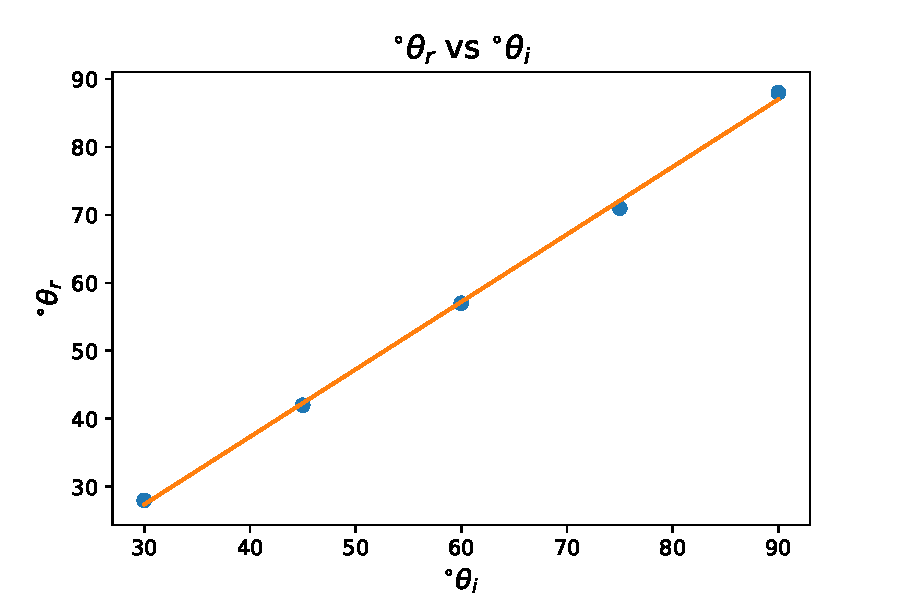
\includegraphics[width=\columnwidth]{img/angulos.pdf}
\caption{\label{fig:img_2} Comparación entre el ángulo del haz de incidencia con respecto al ángulo del haz reflejado.}
\end{figure}

Al realizar un ajuste sobre los puntos de la gráfica de la figura \ref{fig:img_2} se obtiene:
\begin{equation}
    \theta_r = 0.993(\theta_i) - 2.40
\end{equation}
El intercepto del ajuste nos sugiere una fuente de error en el experimento de $-2.40$ grados para cada medida de $\theta_r$, lo cual es relevante ya que el haz reflejado por el espejo en el disco de Harlt era más difuso y por tanto, el ángulo más difícil de medir con exactitud. Por otro lado, la pendiente de la recta es cercana a uno, es decir, ambas variables crecen a la vez en cantidades iguales, que es lo que se espera de acuerdo con las leyes de la reflexión.

La demostración teórica de estos resultados se puede notar en que el rayo incidente, el rayo reflejado
y la normal, se encuentran en un mismo plano; esto produce una relación geométrica entre los ángulos con que incide el rayo y con que es reflejado. Esta afirmación tiene base en las dos primeras leyes leyes de la reflexión, en donde se menciona que la reflexión de luz para espejos planos se denomina reflexión especular; y los rayos incidentes se reflejan con un mismo ángulo. El cumplimiento de esta segunda ley de la reflexión, se deriva del \textit{Principio de Fermat}. Este afirma que la trayectoria real que sigue un rayo de luz entre dos puntos es aquella en la que emplea un tiempo mínimo en recorrerla.\\

\begin{figure}[H]
    \centering
    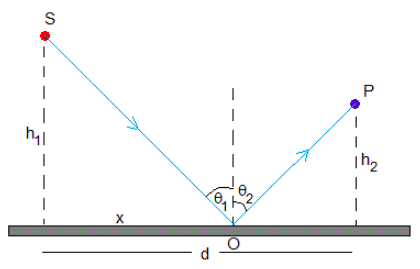
\includegraphics[width=\columnwidth]{img/PF.png}
    \caption{Descripción gráfica del principio de Fermat}
    \label{fig:k1}
\end{figure}

Teniendo en cuenta la figura \ref{fig:k1}. La trayectoria recorrida por el rayo de luz es, $SOP$. Ahora, teniendo en cuenta que:
\begin{itemize}
    \item $x$ es la distancia de $S$ a $O$
    \item $d-x$ es la distancia de $P$ a $O$
    \item $h_1$ es la distancia de $S$ al espejo
    \item $h_2$ es la distancia de $P$ al espejo
\end{itemize}

El tiempo que la luz tarda en hacer el recorrido viene dado por la expresión:

\begin{equation*}
 t = \dfrac{\sqrt{h_1^{2} + x^{2}}}{c} + \dfrac{\sqrt{h_2^{2} + (d - x)^{2}}}{c}   
\end{equation*}

Derivando el tiempo con respecto a $x$ en igualando a $0$, se obtiene:
    
\begin{equation*}
    \dfrac{dx}{dt} = \dfrac{x}{c \sqrt{h_1^{2} + x^{2}}} - \dfrac{d-x}{c\sqrt{h_2^{2} + (d - x)^{2}}}
\end{equation*}
\begin{equation*}
    \dfrac{\sen \theta_{i}}{c} = \frac{\sen \theta_{r}}{c}
\end{equation*}
\begin{equation*}
   \theta_{i}=\theta_{r}
\end{equation*}

\subsection{Experimento: Refracción de luz}
\begin{figure}
\centering
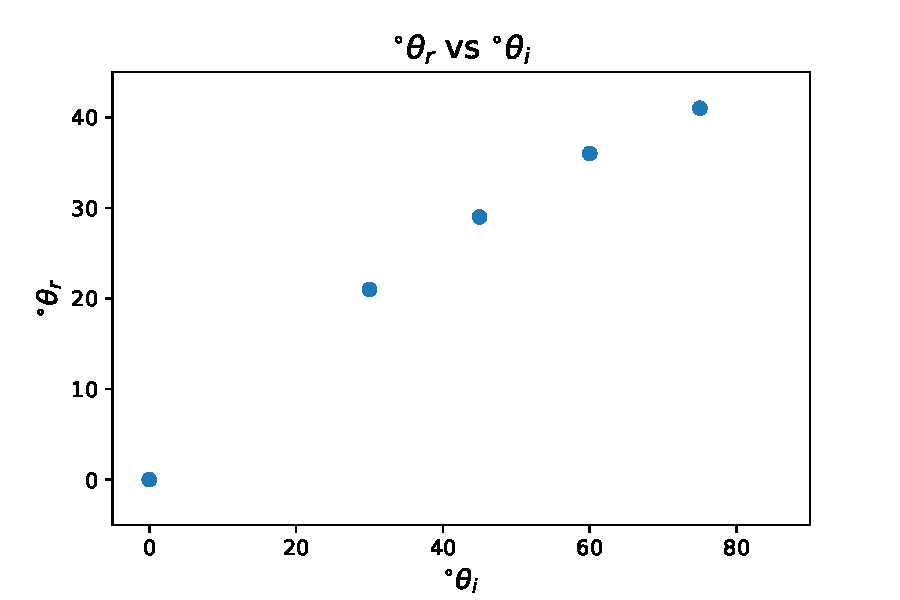
\includegraphics[width=\columnwidth]{img/img2.pdf}
\caption{\label{fig:img_3} Comparación entre el ángulo del haz de incidencia con respecto al ángulo del haz transmitido en un medio material semicircular.}
\end{figure}

Al observar la figura \ref{fig:img_3} se observa una gráfica en la cual las variables no poseen una relación lineal. Luego, la teoría nos sugiere que una de las formas de linealizar esta gráfica es mediante la ley de Snell, revise la ecuación (\ref{eqn:ley_snell}), es decir:
\begin{gather}
    y = \sin{\theta_t}\\
    x = \sin{\theta_i}\\
    \Rightarrow y = \frac{n_1}{n_2}*x 
\end{gather}
De modo que la pendiente de la recta resultante (ver figura \ref{fig:img_4}) corresponderá a la razón entre los índices de refracción de los materiales en la cual se propaga el haz de luz.
\begin{figure}
\centering
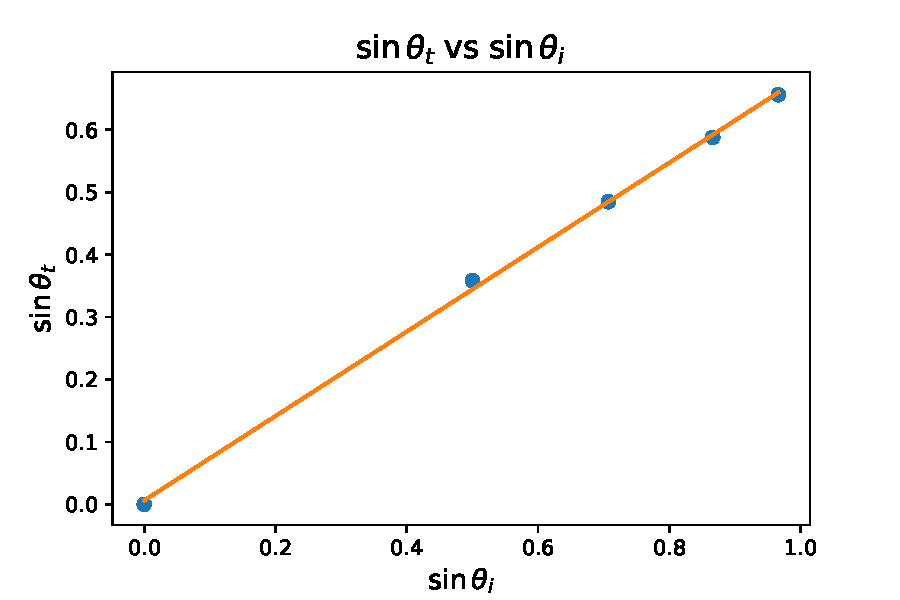
\includegraphics[width=\columnwidth]{img/img3.pdf}
\caption{\label{fig:img_4} Relación entre $\sin{\theta_t}$ vs $\sin{\theta_i}$.}
\end{figure}
Mediante el ajuste de la recta de la figura \ref{fig:img_4} obtenemos que la pendiente:
\begin{gather}
    m = \frac{n_1}{n_2} = 0.676 
\end{gather}
Por otro lado, la literatura propone que el índice de refracción en el aire es de $1.00029$ pero para efectos prácticos se considera como $1$, ya que el aire es un gas evidentemente menos denso que el segundo medio (que es sólido) utilizado en el experimento; luego la velocidad de la luz en este medio es muy cercana a la del vacío. Entonces:
\begin{gather}
    n \approx 1\\
    m = \frac{1}{n_2} = 0.676\\
    \Rightarrow n_2 = \frac{1}{0.676} = 1.48
\end{gather}
Este índice de refracción es cercano a índices de materiales como: el acrílico ($1.49$), el cuarzo fundido ($1.46$) y algunos tipos de vidrios como el vidrio crown ($1.5$), el vidrio fluorado ($1.4$) o el vidrio flint ($1.5$) \cite{eswiki:139589363}.\\

Un detalle curioso en el esquema del montaje (figura \ref{fig:img_1}), es que el haz de luz atraviesa realmente 3 medios: primero el aire, luego el material sólido y nuevamente el aire. Cuando el haz cruza el 3er medio (aire) su dirección debería ser igual a la dirección del haz al inicio, pero esto no es lo que ocurre, ya que el haz resultante posee la dirección del haz refractado. Esto se debe esencialmente a la forma semicircular y cóncava de la superficie del material sólido que corrige el ángulo del haz en el 3er medio desplazando el eje normal como suele ocurrir en superficies difusas.
% intercepto 0.00632
\section{Conclusiones}
Se logró concluir que cuando un haz de luz incide sobre una superficie que separa dos medios diferentes, el haz que se refleja y el haz incidente poseen la misma separación angular con respecto a un eje normal a la superficie. Por otro lado, se obtuvo que la dirección de un haz que se propaga por un medio, al atravesar un segundo medio tendrá una dirección angular que necesariamente depende de la razón entre los índices de refracción de los medios materiales y del ángulo del haz incidente, lo cual se sigue teóricamente por la ley de Snell.
% If in two-column mode, this environment will change to single-column
% format so that long equations can be displayed. Use
% sparingly.
%\begin{widetext}
% put long equation here
%\end{widetext}



\bibliography{report_physics}
\end{document}